\documentclass[]{article}
\usepackage{ctex}
\usepackage{graphics}
\usepackage[colorlinks,linkcolor=black,anchorcolor=blue,citecolor=green,CJKbookmarks=True]{hyperref}
\usepackage{amsmath}
\usepackage{CJK}
\usepackage{indentfirst}
\usepackage{amsmath}
\usepackage{mathrsfs}
\usepackage{eufrak}
\usepackage{geometry}



\geometry{a4paper,scale=0.8}

%opening
\title{计算机视觉论文阅读集合}
\author{wanghao}

\begin{document}

\maketitle
\tableofcontents
\newpage
\hypersetup{hidelinks}

\section{图像分类}
\section{目标检测}
\subsection{\href{./papers/Rich feature hierarchies for accurate object detection and semantic segmentation.pdf}{Rich feature hierarchies for accurate object detection and semantic segmentation}}

\subsubsection{模型框架}
R-CNN分为三个模块。

\textbf{提出候选框}。 
文章采用selective search方法,对一张图片计算出若干个边界框。

\textbf{特征抽取}。 
将边界框在原图中对应的区域都resize成227*227大小的,然后将提取出来的区域输入到CNN特征提取网络中,最终输出4096维的特征向量。

\textbf{SVM线性分类}。
SVMs的输入为4096维的特征向量,输出为N维的分数向量。N表示可识别物体的种类,分数表示图像是该类物体的可能性。该SVMs由N个二分类SVM构成,每个SVM都对应了一个类别。

虽然文章中宣称只有三个模块,但是实际上还有一个模块。

\textbf{边界框回归}。
每类物体都有一组回归器用于修正预测框的位置。当候选框经过SVMs打分后,再通过对应类的回归器,修正候选框位置。

\subsubsection{模型训练}

模型采用分步的训练方法。

\textbf{CNN特征提取网络}。

将已经训练好的用于图像分类的CNN网络的分类层修改为N+1(N表示物体种类,1表示背景类)路,然后进行微调。与真实框有>=0.5 IoU的候选框作为这个框类别的正样本,其余的作为负样本。注意如果一个候选框包含了两个的真实框,则取最大IoU值的真实框作为改候选框的正样本。每次SGD迭代微调,都采样32个正样本,96个负样本作为一个mini-batch。

\textbf{SVM线性分类}

对每类物体都训练一个SVM二分类器。对每一类的SVM分类器来说,将真实框作为正样本,将候选框与所有该类真实框的IoU都$\leq \theta$的作为负样本。最优的$\theta$值用搜索的方法找出来(实验结果为0.3)。

\textbf{边界框回归}

训练集由$\{P^i,G^i ,\phi (P^i )\}$组成,${P^i}=(P^i_x,P^i_y,P^i_w,P^i_h),{G^i}=(G^i_x,G^i_y,G^i_w,G^i_h)$ 。$G^i$是距离$P^i$最近的真实框,并且他们的IoU$\geq0.6$。如果不存在这样的真实框,则该候选框会被丢弃。每一组训练器都由四个线性回归器组成,$d_*(P)=\{d_x(P),d_y(P),d_w(P),d_h(P)\}$,$d_*(P) = w_*^T\phi(P)$,$\phi(P)$表示CNN网络提取出来的特征。预测的$\hat{G}_*$由以下方程构造出来:
\begin{align}
\hat{G}_i^x & =  P_i^wd_x(P) + P_i^x \\
\hat{G}_i^y & =  P_i^hd_y(P) + P_i^y \\
\hat{G}_i^w & =  P_i^w\exp(d_w(P)) \\
\hat{G}_i^h & =  P_i^h\exp(dh(P)) 
\end{align}
定义回归器$d_*(P)$的目标为$t_*$,则:
\label{t*}
\begin{align}
	t_x&=(G_x - P_x)/P_w \\
	t_y&=(G_y - P_y)/P_h \\
	t_w&=\log(G_w / P_w)  \\
	t_h&=\log(G_h / P_h)
\end{align}
目标函数为:
\begin{equation}
\mathbf{w_*}=\mathop{\arg\min}_{\hat{\mathbf{w}}_*} \sum_{i}^{N}(t_{*}^{i}-\hat{\mathbf{w}}_*^{\text{T}} \phi_5 (P^i ))+\lambda || \hat{\mathbf{w}}_* ||
\end{equation}

\textbf{注意},CNN和SVM的正负样本的定义是不同的。SVMs是重新训练的,不需要微调。所以正负样本的定义不需要跟CNN训练时相同。作者发现用这个正负样本定义比用微调的正负样本定义的效果要好。作者认为正负样本的定义不同并不重要,关键是用于微调的数据是有限的。如果只把真实框作为正样本,可能会导致微调网络时过拟合。通过将那些IoU在[0.5,1)之间的
候选框(jittered examples)作为正样本,可以把正样本的数据量扩大30倍。值得注意的是,把这些抖动的样本作为正样本可能不是一个最好的选择,因为没有用一个精确的位置去微调网络。

为什么在网络最后使用SVMs进行分类呢?作者发现使用SVMs的效果比使用原始的全连接层效果要好。作者猜测是正样本的设置策略导致了这个问题。作者认为如果有足够的检测训练数据,整个训练过程的正负样本就可以简单地统一为SVMs的样本设置策略,并且可以把SVM变为全连接层。这样就能简化整个R-CNN的训练过程。

\subsubsection{模型测试}
ss生成2000个候选框,然后将框中的图像reisze成227*227的RGB图像,进入CNN网络提取出每个候选框对应的特征,然后将特征送入SVMs分类器,得到属于每个类的得分,判断出该候选框属于哪个类,最后再使用NMS算法,生成最后的边界框集合。

\subsection{\href{./papers/Fast R-CNN.pdf}{Fast R-CNN}}
Fast R-CNN融合了SPPnet和R-CNN的特点,并做了一些改进。作者在R-CNN的基础上,根据SPPnet提出了RoI Layer,然后合并了框的回归与分类计算,最终得到了Fast R-CNN。与SPPnet和R-CNN相比具有以下优点:
\begin{enumerate}
	\item 对比SPPnet,R-CNN有更高的检测质量。
	\item 训练是单阶段,不需要分为很多步,使用了多任务损失。
	\item 训练步骤可以更新所有的网络层参数,对比SPPnet。
	\item 不需要硬盘保存特征。
\end{enumerate}
\subsubsection{模型框架}
Fast R-CNN主要分为四个模块。

\textbf{提出候选框}。使用ss方法,与R-CNN中的提出候选框模块相同。

\textbf{特征图计算}。直接将原始图片输入CNN特征提取网络,获取整个图片对应的特征映射图。

\textbf{候选框特征提取}。将在原图上的候选框$(x,y,w,h)$映射到特征图($M \times N$)上去,然后截取框内的特征,池化后输出固定维度的特征,将该层称为 RoI pooling layer。假设$(x,y,w,h)$为候选框,我们需要计算出该候选框在feature map上的位置$(x^{'},y^{'} ,w^{'} ,h^{'})$。假设候选框$(x,y,w,h)$由左上角$(x_1,y_1)$和右下角$(x_2,y_2)$两个点构成,其中心点为$(\bar{x},\bar{y})$。我们只需要分别对$(x_1,y_1),(x_2,y_2)$找到在feature map上能感受到他们的点$(x_1^{'} ,y_1^{'})$,$(x_2^{'} ,y_2^{'})$。$(x_1^{'} ,y_1^{'})$和$(x_2^{'} ,y_2^{'})$即可确定$(x^{'},y^{'} ,w^{'} ,h^{'})$。feature map 上的每个点都能映射到原始图上去,可看成该映射点为中心的窗口做卷积得到。由于原始图上的点$(x_i,y_i)$可能被feature map上的多个点$(x_j^{'},y_j^{'})$感受到,我们需要选择一个点作为它的感受点,并且选择的这个点的映射点离$(x_i,y_i)$最近。$(x_1^{'} $和$y_1^{'})$和$(x_2^{'} ,y_2^{'})$都按照上述方法确定。

假设核大小为$k \times k$,步长为$s$,填充为$p$,$k$为奇数。

feature map到原图映射点的计算方法。设第$i+1$层上的点为$(x^{'} ,y^{'})$,其在第$i$层的映射点为$(x,y)$,则:
\begin{align}
x=x^{'}*s+\lfloor k/2 \rfloor - p \\
y=y^{'}*s+\lfloor k/2 \rfloor - p 
\end{align}

原图到feature map感受点的计算方法。设第$i$层的点为$(x,y)$,其在第$i+1$层上的感受点为$(x^{'} ,y^{'})$,则:
\begin{align}
x^{'}=(x+p-\lfloor k/2 \rfloor)/s \\
y^{'}=(y+p-\lfloor k/2 \rfloor)/s
\end{align}
感受点的计算与映射点的计算是互逆的,但是映射点一定能得到整数值,感受点可能计算出浮点数。而浮点坐标是在这里是不存在的,再对浮点坐标取整即可。

在\href{./papers/Fast R-CNN.pdf}{Fast R-CNN}中,作者强行令$p=\lfloor k/2 \rfloor $,最终得到:
\begin{align}
	x^{'}=x/s \\
	y^{'}=y/s
\end{align}
假设在feature map前有$n$个卷积层和池化层,每层的步长为$s_i$,feature map上的点为$(x^{'} ,y^{'} )$则:
\begin{align}
	x^{'}=x/S=x/\prod_{i=1}^{n}s_i \\
	y^{'}=y/S=x/\prod_{i=1}^{n}s_i 
\end{align}
由于可能得到浮点数,作者向候选框的中心做了偏移,即得到:
\begin{align}
x_1^{'}=\lfloor x_1/S \rfloor +1\\
y_1^{'}=\lfloor y_1/S \rfloor +1\\
x_2^{'}=\lfloor x_2/S \rfloor -1\\
y_2^{'}=\lfloor y_2/S \rfloor -1
\end{align}
由于$k\geq 1$,所以上述计算得到的点一定可以感受到要感受的点。窃以为用$x_1^{'}=\lceil x/S \rceil,x_2^{'}=\lfloor x_2/S \rfloor$更好(:。

找到在feature map上的特征框$(x^{'},y^{'} ,w^{'} ,h^{'})$后,进行最大池化。对任意大小的特征框都生成固定大小($H \times W$)的特征向量(在VGG16中,$H=W=7$)。

\textbf{分类与边界框回归}。该模块对应了两个任务,包括框的分类和回归。固定维度的特征经过一系列全连接层后分为两个分支,一个分支经过softmax输出每个类别(加上背景)的概率,一个分支对每一类输出4个回归值$(t_x,t_y,t_h,t_w)$,$t_*$的定义与R-CNN中是相同的,利用候选框与真实框计算出$t_*$。

\subsubsection{模型训练}
\label{Fast R-CNN}
Fast R-CNN将R-CNN的三个训练部分合成了一个整体。可以更新所有层的参数(R-CNN和SPPnet无法根据SVM的loss,更新卷积层的参数),可以实现端到端的训练。不需要将特征缓存在硬盘中。

\textbf{数据生成}。
每个mini-batch,作者随机取出2张图片,然后在2张图片上共采样出128个候选框,每张图片采样出64个候选框。将$IoU \geq 0.5$的作为正样本,将$IoU$在$[0.1)$的作为负样本,每个mini-batch生成的正负样本比例为1:3。训练时,图片以0.5的概率随机水平翻转。

\textbf{损失函数}。
Fast R-CNN使用了多任务损失函数$L(p,u,t^{u},v)$:
\begin{align}
	L(p,u,t^{u},v)&=L_{cls}(p,u)+\lambda[u\geq1]L_{loc}(t^u,v)\\
	L_{cls}(p,u)&=-\log p_u\\
	L_{loc}(t^u,v)&=\sum_{i\in {x,y,w,h}} \text{smooth}_{L1}(t^u_i - v_i)\\
	\text{smooth}_{L1}(x)&=
	\left\{
	\begin{aligned}
	0.5x^2\\
	|x|-0.5
	\end{aligned}
	\right.
	\end{align}
$p$是softmax输出的$K+1$维类别概率矩阵,$u$表示该框的真实类别,$v$表示框的真实偏移,$t^u$表示框的预测偏移(定义与\ref{t*}中相同)。损失函数由类别损失和位置损失两部分构成,当真实类别为前景($u\geq 1$)时,位置损失有效,当真实类别为背景($u=0$)时,位置损失无效。

\textbf{注意}。1. Fast R-CNN中的三个部分是统一训练的,正负样本的策略是相同的,这与R-CNN中有很大不同。2. Fast R-CNN中类别分类使用的是softmax,而R-CNN中使用的是SVM。3.Fast R-CNN采用的是联合训练方式,而R-CNN中CNN网络微调、框的分类和回归的训练是分开的。作者通过实验证明联合训练的方式效果比分步训练好,softmax的效果始终比SVM好一点。使用更严格负样本策略的SVM在S和M的模式的Fast-RCNN的效果好,而在L模式下,联合训练的效果比使用更严格负样本策略的SVM好。
\subsubsection{模型测试}
ss生成大概2000个候选框,经过整个网络输出每个框的类别和位置,再使用NMS输出结果。

\subsection{\href{./papers/Faster R-CNN-Towards Real-Time Object.pdf}{Faster R-CNN-Towards Real-Time Object}}
作者在Fast R-CNN的基础上,用RPN网络代替了ss算法。
\subsubsection{模型框架}
\textbf{Fast R-CNN网络}。
除去ss算法部分的Fast R-CNN结构。

\textbf{RPN网络}。RPN网络主要用于生成候选框,与ss的作用是相同相同的。网络结构组成:feature map以前的网络结构部分+$n\times n$的卷积层+两个分离的$1\times 1$卷积层(分别用于anchors的分类和回归)。RPN网络实际上以feature map层上的每个点为中心,将这些点映射到原图上去,每个点都有大小相同、形式相同的多个框。将这些框作为默认框,进行分类和回归,生成效果更好的候选框。

Anchors。所谓的anchors实际上就是在原图上画的一些默认框,这些默认框可以看成滑动窗口在一些点上移动构成的,而这些点是从feature map上映射下来的。假设feature map上每个点对应了$k$个框,文章中默认使用了3种大小,3种长宽比,则每个点产生$k=9$个点。假设feature map的大小为$W*H$,则共产生$WHk$个anchors。

Fast R-CNN和RPN共享了feature map层之前的网络结构。

\subsubsection{模型训练}
相较Fast R-CNN,Faster R-CNN增加了一个RPN网络的训练。

\textbf{4步联合训练方法}。1.训练RPN网络,用预训练好的模型初始化参数。2.训练一个分开的Fast R-CNN网络,使用RPN网络生成的框,用预训练好模型初始化参数。此时,两个网络没有共享参数。3.再次训练RPN网络,用第2步训练好的Fast R-CNN的参数初始化RPN共享部分的网络参数,然后固定共享部分的参数,只微调RPN独有的网络部分。此时,RPN和Fast R-CNN共享了feature map前网络的参数。4.再次训练Fast R-CNN网络,固定共享部分的参数,微调Fast R-CNN独有的网络部分。

\textbf{RPN网络训练}。
RPN的训练是端到端的。每个 mini-batch 的训练数据都是从一张图片生成的。一张图片的所有anchorts包含了大量的负样本和少量的负样本,因此在训练的时候,我们不能使用所有的anchors,否则会导致损失函数偏向负样本。每次mini-batch 采样256个anchors,正负样本比例设置为$1:1$,若正样本不足,则用负样本填充。正样本规则:1.和一个真实框具有最高的IoU,2.和任意一个真实框的IoU$\ge 0.7$。负样本规则:和所有框的IoU都$\le 0.3$。用$(0,0.01)$的高斯分布初始化RPN独有的层,用预训练好的模型初始化其他的。损失函数如下:
\begin{equation}
L(\{p_i\},\{t_i\})=
\frac{1}{N_{cls}}\sum_{i}L_{cls}(p_i,p_i^*)\\
+\lambda \frac{1}{N_{reg}}\sum_{i}p_i^* L_{reg}(t_i,t_i^*)
\end{equation}
$L_{cls}(p_i,p_i^*)$和$L_{reg}(t_i,t_i^*)$跟\ref{Fast R-CNN}中是类似的,分别代表对数损失和回归损失,$\lambda$设为10。

\textbf{Fast R-CNN网络训练}。与 \ref{Fast R-CNN}是类似的。不同的地方在于RPN网络可能产生的候选框比ss算法的多,而RPN中的候选框相互之间可能有很高的IoU。训练时,为了减少冗余计算,我们对RPN的候选框做了一个NMS(阈值设为0.7),最终大概2000个候选框。RPN网络可能生成了超出图片边界的框,对于这种框直接忽略。
\subsubsection{模型测试}
与Fast R-CNN类似。注意RPN生成的候选框可能超出了边界,对于这种框需要通过去除超出边界的部分,修正框的位置。
\subsection{\href{./papers/You Only Look Once-Unified Real-Time Object Dectection.pdf}{You Only Look Once-Unified Real-Time Object Dectection}}
\subsubsection{模型框架}
\subsubsection{模型训练}
\subsubsection{模型测试}
\subsection{\href{./papers/SSD Single Shot MultiBox Detector.pdf}{SSD:Single Shot MultiBox Detector}}
\subsubsection{模型框架}
\subsubsection{模型训练}
\subsubsection{模型测试}

\section{目标追踪}

目前在目标追踪领域识别效果最好的是Siamese Networks系列的模型,并且它的运行速度远远超过了人眼所需的帧率。

\subsection{\href{./papers/Fully-Convolutional Siamese Networks.pdf}{Fully-Convolutional Siamese Networks}}
\label{SiamFC}

本文提出了一个新的全卷积孪生网络,在 ILSVRC15 上达到了最优。
\subsubsection{模型框架}
该模型由一个Siamese network和一个cross-correlation 层组成。最终输出一个 score map,在score map中取最大的值对应的位置,即为目标位置。

\textbf{Siamese network}。实际上就是一个全卷积神经网络,用于提取图像的特征。该网络输入两张图像,同时经过同一个卷积神经网络,输出两个特征图,将该网络抽象为函数$\varphi$。两张图像一个作为 exemplar image $z$,一个作为 candidate image $X$,最终生成$\varphi (z)$和$\varphi (X)$。

\textbf{Cross-correlation}。实质上就是一个卷积层,将$z$视为卷积核,步长为1,在$X$上做卷积,最终生成一个score map,其上的每个点表示是该物体的得分值。

模型框架如图~\ref{siamFC_architecture} 所示。

\begin{figure}
	\centering
	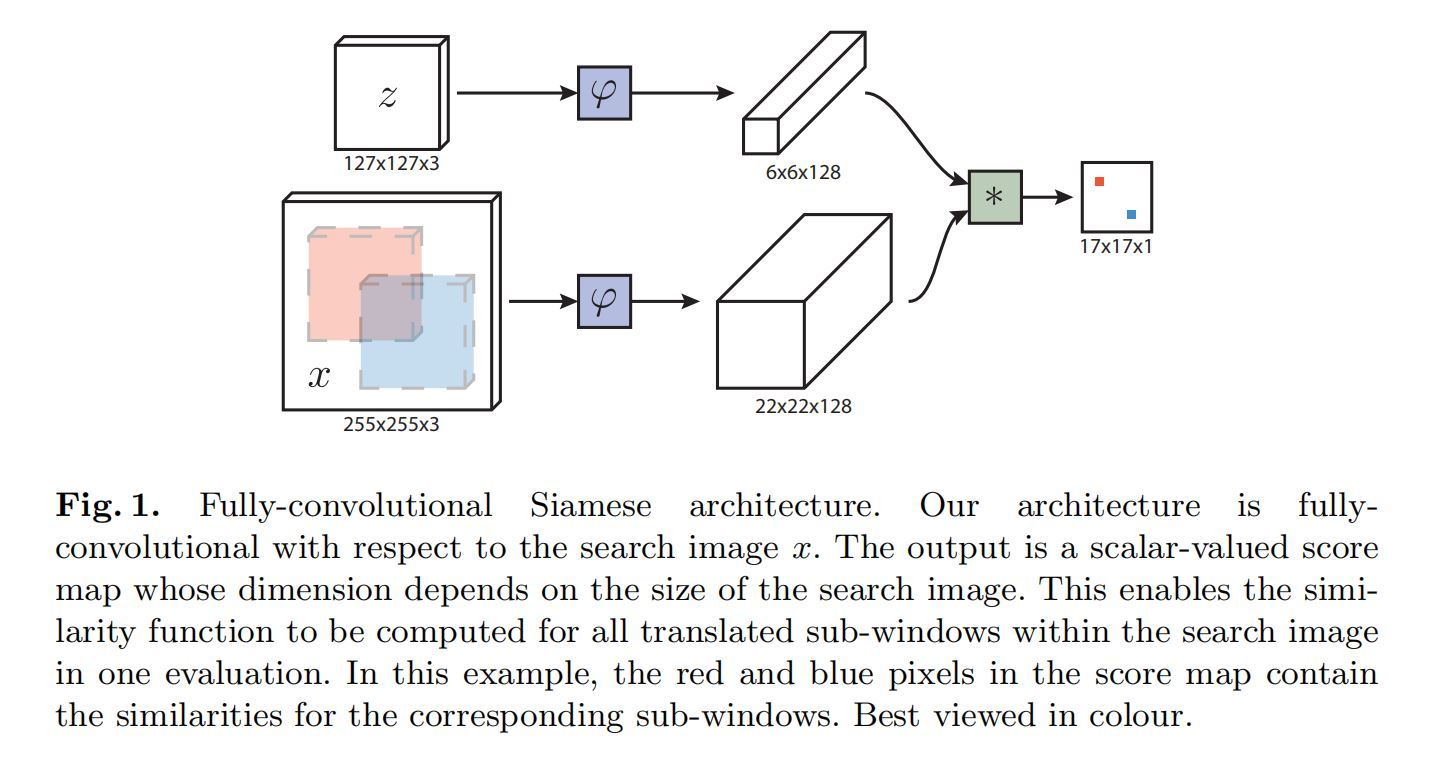
\includegraphics[width=0.7\linewidth]{./images/siaFC.jpg} 
	\caption{siamFC 框架}
	\label{siamFC_architecture} 
\end{figure}

\subsubsection{模型训练}
\textbf{数据生成}。每次从一段视频中抽取出两帧图像,两张图像均包含目标物体。$z$的大小是$127\times 127$,$X$的大小是$255\times 255$。$z$和$X$以相同的方式生成,假设边界框大小为$(w,h)$,以目标物体为中心扩增上下文(就是原图像)边距$p=(w+h)/4$,然后再对$(w+2p,h+2p)$用各通道均值做一个padding,使其达到$z$或$X$需要的大小。对score map上的每个点都要生成一个label,当该点与目标中心的距离不大于$R$时,设为正值$1$,否则为$-1$。

\textbf{损失函数}。对最终生成的score map计算损失值。
\begin{equation}
	L(y,v)=\frac{1}{|\mathcal{D}|}\sum_{u\in \mathcal{D}}l(y[u],v[u])
\end{equation}
$y$表示真实值,$v$表示计算出来的值,$u$表示score map上的点,$\mathcal{D}$表示score map,$L$表示损失。

单个点的损失函数:
\begin{equation}
	l(y,v)=\log (1+\exp(-yv))
\end{equation}

\subsubsection{模型测试}
测试时输入一段视频和第一帧中目标的位置。用上述的方法抽取出第一帧的$z$,只算一次$\varphi (z)$。每次的搜索区域都是以上一帧目标中心为中心,大小为上一帧目标大小的四倍(实际上就固定是$255 \times 255$了,因为能检测到的目标大小只能是$127\times 127$)。最后生成的score map大小始终为$17 \times 17$,然后对这个socre map做一个三线性插值,生成$272 \times 272$大小的score map,然后再取最大值,至于为什么要这么干,当然是作者测出来这么干效果好了(:。此外,作者假设在相邻的帧中,物体的位置,形状,大小等都是相似的,对于较大的变化都有一个惩罚,为了应对物体的尺度多样性,作者用五种尺度去搜索,。

\subsection{\href{./papers/High Performance Visual Tracking with Siamese Region Proposal Network.pdf}{High Performance Visual Tracking with Siamese Region Proposal Network}}
该论文实际上是siamFC模型和RPN网络的合体版本。
\subsubsection{模型框架}
该模型由一个孪生神经网络和RPN网络组成,输出每个默认框的位置修正值和正负概率。


\textbf{Siamese network}。一个全连接神经网络,用于提取图像特征,与 \ref{SiamFC}中类似。

\textbf{RPN}。与\ref{Fast R-CNN}中的RPN网络类似,此时将$\varphi(X)$作为输入的feature map,然后分为两路一路用于分类,一路用于回归。$\varphi(z)$作为卷积核,同样分为两路一路用于分类,一路用于回归。在分类和回归两个分支中,$\varphi(X)$和$\varphi(z)$都先经过一个卷积层,然后两者再做互相关操作(互相关此时为卷积操作与\ref{SiamFC}相同)。

模型框架如图 \ref{SiamRPN_architecture} 所示。
\begin{figure}
	\centering
	\includegraphics[width=0.9\linewidth]{./images/siamRPN.jpg} 
	\caption{SiamRPN 框架}
	\label{SiamRPN_architecture} 
\end{figure}

\subsubsection{模型训练}
\subsubsection{模型测试}

\subsection{\href{./papers/Distractor-aware Siamese Networks for Visual.pdf}{Distractor-aware Siamese Networks for Visual}}
\subsubsection{模型框架}
\subsubsection{模型训练}
\subsubsection{模型测试}

\section{实例分割}
\subsection{Mask R-CNN}

\section{对抗攻击}
\section{其他}


\end{document}

